% FIG ch07-03a V1 error markers (language-neutral)
\definecolor{ch07err}{HTML}{C0392B}
\makeatletter
\@ifundefined{chsevenerrmark}{%
\newcommand{\chsevenerrmark}[2][]{%
  \tikz[baseline=(char.base)]{%
    \node[shape=circle, fill=ch07err, text=white, inner sep=1.5pt,
      font=\fontsize{7}{7}\selectfont\bfseries, #1] (char) {#2};}}%
}{}
\makeatother
\begin{tikzpicture}
  \node[anchor=south west, inner sep=0] (img) at (0,0)
    {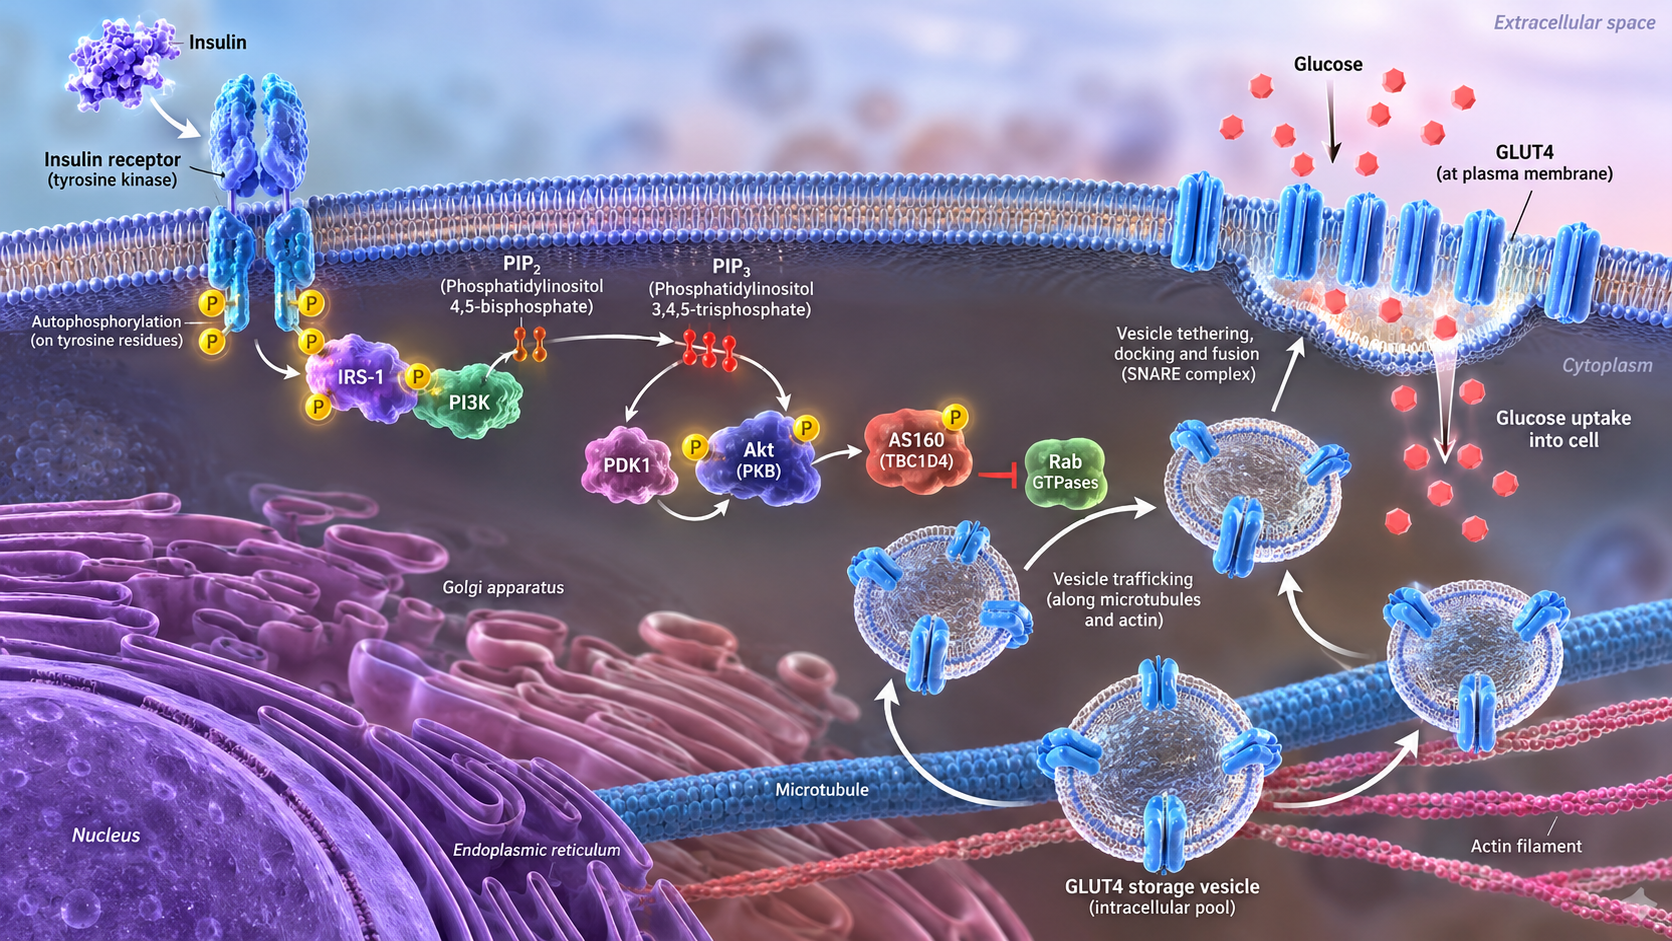
\includegraphics[width=\linewidth]{figures/ch07/ch07-03a-v1-vague.png}};
  \begin{scope}[x={(img.south east)}, y={(img.north west)}]
    \node at (0.14, 1-0.18) {\chsevenerrmark{1}};
    \node at (0.72, 1-0.22) {\chsevenerrmark{2}};
    \node at (0.50, 1-0.35) {\chsevenerrmark{3}};
    \node at (0.38, 1-0.55) {\chsevenerrmark{4}};
    \node at (0.55, 1-0.72) {\chsevenerrmark{5}};
    \node at (0.22, 1-0.48) {\chsevenerrmark{6}};
    \node at (0.82, 1-0.40) {\chsevenerrmark{7}};
  \end{scope}
\end{tikzpicture}
